% EE604 course project write-up, typeset with the CVPR author kit (2022/2023 style files:
% cvpr.sty + ieee_fullname.bst), as required by the course guidelines.
\documentclass[10pt,twocolumn,letterpaper]{article}

\usepackage{cvpr}              % camera-ready mode so that author names are shown
\usepackage{graphicx}
\usepackage{amsmath}
\usepackage{amssymb}
\usepackage{booktabs}
\usepackage{multirow}
\usepackage{xcolor}
\usepackage{tikz}
\usetikzlibrary{arrows.meta,positioning,calc}
\usepackage{listings}
\usepackage{enumitem}
\usepackage[pagebackref,breaklinks,colorlinks,allcolors=blue!60!black]{hyperref}
\usepackage[capitalize]{cleveref}
\crefname{section}{Sec.}{Secs.}
\crefname{table}{Tab.}{Tabs.}
\crefname{figure}{Fig.}{Figs.}

\lstset{basicstyle=\ttfamily\fontsize{6.2}{7.0}\selectfont, breaklines=true,
        columns=fullflexible, keepspaces=true, showstringspaces=false,
        commentstyle=\color{black!55}, keywordstyle=\color{blue!60!black},
        language=Python, frame=none, xleftmargin=0pt}

% Auto-generated by experiments/make_tables.py -- do not edit by hand
\newcommand{\rhoMzero}{0.823}
\newcommand{\rhoMzeroNoAlign}{0.614}
\newcommand{\rhoMzeroFixed}{0.931}
\newcommand{\rhoMone}{0.938}
\newcommand{\rhoMthree}{0.947}
\newcommand{\maeMone}{0.45}
\newcommand{\maeMthree}{0.45}
\newcommand{\kdWrong}{58.3}
\newcommand{\nmeFitInner}{3.95}
\newcommand{\nmeHandInner}{4.23}
\newcommand{\nmeFitJaw}{8.13}
\newcommand{\nmeHandJaw}{10.11}
\newcommand{\nmeFitInnerMed}{3.13}
\newcommand{\shrinkGlobal}{12.4}
\newcommand{\shrinkMouth}{26.7}
\newcommand{\shrinkBrows}{1.9}
\newcommand{\pBrows}{0.08}
\newcommand{\silentCleanOne}{5.8}
\newcommand{\silentCleanTwo}{4.9}
\newcommand{\silentCleanThree}{4.0}
\newcommand{\covCleanThree}{89.7}
\newcommand{\accCleanThree}{42.0}
\newcommand{\silentPoolOne}{8.1}
\newcommand{\silentPoolTwo}{3.4}
\newcommand{\silentPoolThree}{3.6}
\newcommand{\covPoolThree}{63.2}
\newcommand{\accPoolThree}{21.0}
\newcommand{\silentBlurOne}{14.4}
\newcommand{\silentBlurTwo}{2.7}
\newcommand{\silentBlurThree}{2.3}
\newcommand{\covBlurThree}{35.6}
\newcommand{\accBlurThree}{5.2}
\newcommand{\silentDownOne}{9.2}
\newcommand{\silentDownTwo}{1.8}
\newcommand{\silentDownThree}{1.9}
\newcommand{\covDownThree}{33.4}
\newcommand{\accDownThree}{4.0}
\newcommand{\driftPoolOne}{0.076}
\newcommand{\driftPoolThree}{0.054}
\newcommand{\driftPoolZero}{0.070}
\newcommand{\driftReduction}{29}
\newcommand{\rotNoAlignMax}{3.67}
\newcommand{\rotMthreeMax}{0.052}
\newcommand{\detBlurEight}{79.0}
\newcommand{\detMin}{79.0}
\newcommand{\rhoYawRef}{0.91}
\newcommand{\rhoYawRefAcc}{0.75}
\newcommand{\rhoYawMthree}{0.96}
\newcommand{\yawLow}{1.20}
\newcommand{\yawHigh}{5.50}
\newcommand{\rhoMirrorNme}{0.59}
\newcommand{\aurcRandom}{3.37}
\newcommand{\aurcMirror}{2.99}
\newcommand{\aurcGateTwo}{3.29}
\newcommand{\aurcOracle}{2.75}
\newcommand{\gapClosed}{61}
\newcommand{\aurcAsymRandom}{0.442}
\newcommand{\aurcAsymMirror}{0.418}
\newcommand{\aurcAsymGate}{0.437}
\newcommand{\rhoMirrorErr}{0.03}
\newcommand{\pAccept}{42.0}
\newcommand{\pCaution}{47.8}
\newcommand{\pReject}{10.3}
\newcommand{\nmeAccept}{3.03}
\newcommand{\nmeCaution}{4.71}
\newcommand{\occEye}{0.9}
\newcommand{\occNose}{17.5}
\newcommand{\occNoseOther}{8.5}
\newcommand{\occMouth}{18.4}
\newcommand{\occMouthOther}{2.2}
\newcommand{\alphaIndex}{0.467}
\newcommand{\trainMedian}{2.14}
\newcommand{\runtime}{46}
\newcommand{\nTrainOk}{810}

\newcommand{\repo}{\url{https://github.com/pruthav23/Face-Symmetry-Measurement}}

\def\cvprPaperID{EE604}
\def\confName{EE604}
\def\confYear{2026}

\begin{document}

\title{Face Symmetry Measurement: A Quality-Aware, Mirror-Consistent\\
Facial Asymmetry Analysis System}

\author{
Ankit Yadav (230150)\quad Ashish Porwal (230229)\quad Mahi Mittal (230617)\\
Pankaj Kumar (230733)\quad Prutha Vinay (230807)\\
EE604 Image Processing, Course Project, IIT Kanpur\\
{\small Code: \repo}
}

\maketitle

\begin{abstract}
Public facial-symmetry tools take a single 2D photo, detect landmarks, reflect them
about a midline and always return a score, even when the photo cannot support one.
We build a system that accepts one face photo and returns a 2D geometric asymmetry
measure (global and per region) only when it is trustworthy, together with an
accept/caution/reject decision and its reasons. The method has three parts:
(i) asymmetry measured with fixed anatomical left/right pairs and a \emph{fitted}
symmetry axis, rather than nearest-neighbour matching about an assumed vertical midline;
(ii) a \emph{mirror test}, which runs the landmark detector on the photo and on its
mirror image and compares the two results, giving a label-free check of landmark
reliability and averaging out any left/right detector bias;
(iii) a quality gate on face size, sharpness, exposure, head pose and mirror
consistency, with thresholds set on a training split.
Since no dataset contains true symmetry labels, we evaluate against the same measure
computed from human-annotated landmarks (LFPW/300-W, 224 test images) and under 26
controlled perturbations (5{,}824 perturbed images).
The fitted-axis measure agrees far better with this annotation-based reference than a
re-implemented public baseline (Spearman $\rho$ \rhoMthree{} vs.\ \rhoMzero{}); the
baseline's KD-tree matching pairs \kdWrong\% of points with the wrong anatomical
partner. The mirror test ranks images by landmark error without ground truth
($\rho$ = \rhoMirrorNme{}), and mirror averaging cuts score drift under perturbation by
\driftReduction\%. The gate reduces silent failures (scores reported with error
$>$1\% of the inter-ocular distance) from \silentPoolOne\% to \silentPoolThree\%.
We also find that on in-the-wild photos the measured 2D asymmetry follows head yaw
almost one-to-one ($\rho$ = \rhoYawRef{}), even when computed from expert annotations.
This means pose gating is essential, not optional.
\end{abstract}

\section{Introduction}
\label{sec:intro}

Bilateral facial symmetry is measured in orthodontics and maxillofacial
surgery~\cite{berlin2014asymmetry2d}, in outcome assessment after facial plastic
surgery~\cite{varghaei2025aesthetic}, and in face analysis research~\cite{liu2003asymmetry}.
Dense face-landmark detectors such as MediaPipe Face
Landmarker~\cite{kartynnik2019facemesh,mediapipe_facelandmarker} now run in real time on a
laptop CPU, which has produced easy-to-use public tools that turn one selfie into a
``symmetry score''~\cite{nashokan_facialasymmetry,yousrajnahi_symmetry,irimid}.

\paragraph{Why this is harder than it looks.}
A 2D photo is a projection. A head turned by a few degrees, a tilted camera, blur, poor
lighting or an occluded region all change the measured left--right geometry, and the
landmark detector may itself be biased towards a symmetric template. Most existing tools
return a number for every input, and the one with input checks~\cite{irimid} does not
consider head yaw or pitch. A user cannot tell whether a score of ``2\%'' reflects the
face or the photo. Our experiments show that this is a real, large effect: on LFPW the
asymmetry measured \emph{from expert annotations} rises from \yawLow\% to \yawHigh\% of the
inter-ocular distance as head yaw grows from $<$5$^\circ$ to $\geq$20$^\circ$
(\cref{fig:pose}).

\paragraph{Problem statement.}
\emph{Input:} a single RGB photo containing a face.
\emph{Output:} (a) an accept/caution/reject decision with plain-language reasons;
(b) when not rejected, a normalised global asymmetry $A$ and regional values $A_r$ for
brows, eyes, nose, mouth and jaw, with a mirror-stability band and a per-region
reliability flag; (c) visual overlays and a CSV/JSON export.
\emph{Constraints:} 2D images only; a pre-trained detector and explicit geometry, with no
model training; CPU real time (\runtime\,ms per image); no claims about 3D anatomy,
health, identity or attractiveness.

\paragraph{What is new.}
Landmark detection, mirrored-landmark comparison, regional heatmaps and Streamlit
front-ends all already exist in public code~\cite{nashokan_facialasymmetry,
varghaei2025aesthetic,irimid}, and we do not claim them. Our contributions are:
\begin{enumerate}[leftmargin=*,itemsep=1pt,topsep=2pt]
\item \textbf{A rotation-invariant measure with correct correspondence.} We pair the
478 MediaPipe vertices using the exactly symmetric canonical face model, map them to the
standard 68-point layout with a correspondence fitted on a training split and constrained
to be mirror-consistent, and fit the symmetry axis by least squares. We quantify why this
matters: the reflected nearest-neighbour (KD-tree) matching used in prior
tools~\cite{nashokan_facialasymmetry,varghaei2025aesthetic} picks the wrong anatomical
partner for \kdWrong\% of the points.
\item \textbf{A mirror test for a symmetry measurement.} Horizontal-flip test-time
augmentation is standard in pose and landmark
estimation~\cite{newell2016stacked,wang2020hrnet}, where it is used for accuracy. We use it
differently: \emph{flipping the image cannot change a face's asymmetry}, so the
disagreement between the two detections is a label-free reliability signal, and their
average removes any systematic left/right detector bias from the asymmetry estimate. In
the public symmetry tools we audited (\cref{tab:related}) the score is computed from a
single pass.
\item \textbf{A calibrated quality/pose gate with region validity}, whose thresholds
are fixed a priori or set on training data only. It is evaluated as \emph{selective
measurement}~\cite{geifman2017selective}: how many unreliable scores it prevents and how
much coverage it costs.
\item \textbf{An evaluation protocol without symmetry labels.} No public dataset has
ground-truth symmetry. We compare detector-based measurements with the identical measure
computed from expert landmark annotations, and run 26 controlled perturbations. This
gives the findings above, plus two that matter in practice: detector-based asymmetry is
shrunk towards symmetry (by \shrinkGlobal\% overall, \shrinkMouth\% at the mouth), and
the mirror test does \emph{not} detect an occluded eye.
\end{enumerate}

\section{Related Work}
\label{sec:related}

\paragraph{Facial landmark localisation.}
Benchmarks such as LFPW~\cite{belhumeur2011lfpw} and 300-W~\cite{sagonas2013_300w,
sagonas2016_300w} (68 points) and WFLW~\cite{wu2018lab} (98 points, with pose, expression,
illumination, make-up, occlusion and blur subsets) drove accurate in-the-wild alignment.
MediaPipe Face Mesh / Face Landmarker~\cite{kartynnik2019facemesh,lugaresi2019mediapipe,
mediapipe_facelandmarker} regresses 468 surface vertices (+10 iris points) of a fixed
canonical topology and a head-pose transformation matrix in real time on CPU. It returns
no per-landmark confidence (its \texttt{visibility} and \texttt{presence} fields are empty);
this gap is what motivated our mirror test.

\paragraph{Quantifying facial asymmetry.}
Clinical 2D methods compare paired landmarks about a reference
midline~\cite{berlin2014asymmetry2d}. Geometric morphometrics avoids choosing a midline by
superimposing a configuration with its relabelled reflection, separating symmetric and
asymmetric shape components~\cite{klingenberg2002shape,mardia2000symmetry}. Our fitted axis
follows this idea, restricted to a pure 2D reflection. Liu \etal~\cite{liu2003asymmetry}
used image-based asymmetry for identification.

\paragraph{Public symmetry tools.}
Varghaei \etal~\cite{varghaei2025aesthetic} assess facial-plastic-surgery outcomes with
frontal-image filtering, MediaPipe landmarks, KD-tree based mirrored matching and other
morphometrics. Their surgical dataset is not public. The \textit{FacialAsymmetry}
tool~\cite{nashokan_facialasymmetry} implements that symmetry method in Streamlit, with
eye-based alignment, a vertical midline through vertices 33/263, KD-tree matching, seven
regions and a heat map. \textit{Facial-symmetry-estimation}~\cite{yousrajnahi_symmetry}
makes binary symmetric/asymmetric decisions for individual dlib 68-point features with a
fixed tolerance. \textit{irimid}~\cite{irimid} computes anthropometric proportions and a
symmetry index from 20 hand-picked MediaPipe vertex pairs about a vertical median midline.
It also validates inputs with fixed rules on resolution, brightness, sharpness, in-plane
tilt and a span-based occlusion heuristic. \Cref{tab:related} summarises the tools.
Quality checks therefore exist, but none of these tools gates on out-of-plane pose (yaw,
pitch), checks the landmarks themselves, calibrates its thresholds on data, or reports a
quantitative evaluation of its score.

\paragraph{Selective prediction and quality assessment.}
A model that may abstain is evaluated with risk--coverage curves~\cite{geifman2017selective}.
We apply this to measurements. Our image-quality signals are classical: variance of the
Laplacian for focus~\cite{pertuz2013focus} and luminance statistics for exposure.

\begin{table}[t]
\centering\footnotesize
\setlength{\tabcolsep}{2.5pt}
\begin{tabular}{@{}lcccccc@{}}
\toprule
 & Landm. & Pairing & Axis & Regions & Gate & Eval.\\
\midrule
FacialAsym.~\cite{nashokan_facialasymmetry} & MP 478 & KD-tree & vertical & 7 & -- & --\\
Varghaei~\cite{varghaei2025aesthetic} & MP 468 & KD-tree & vertical & -- & frontal & private\\
yousrajnahi~\cite{yousrajnahi_symmetry} & dlib 68 & per feature & landm. line & 7 & -- & --\\
irimid~\cite{irimid} & MP 478 & 20 fixed & vertical & 5 & fixed rules$^{*}$ & --\\
\textbf{Ours} & MP$\to$68 & fixed & \textbf{fitted} & 5 & \textbf{7 signals} & \textbf{LFPW+pert.}\\
\bottomrule
\end{tabular}
\caption{\textbf{What existing public implementations do} (from their READMEs and code,
5~Nov~2026). ``Eval.'': quantitative evaluation reported. $^{*}$resolution, brightness,
sharpness, roll, occlusion heuristic; no yaw/pitch. None of the tools checks landmark
consistency (our mirror test).}
\label{tab:related}
\end{table}

\section{Proposed Method}
\label{sec:method}

% Overview of the proposed quality-aware measurement (M3). Drawn in TikZ so it is editable.
\begin{figure*}[t]
\centering
\resizebox{\textwidth}{!}{%
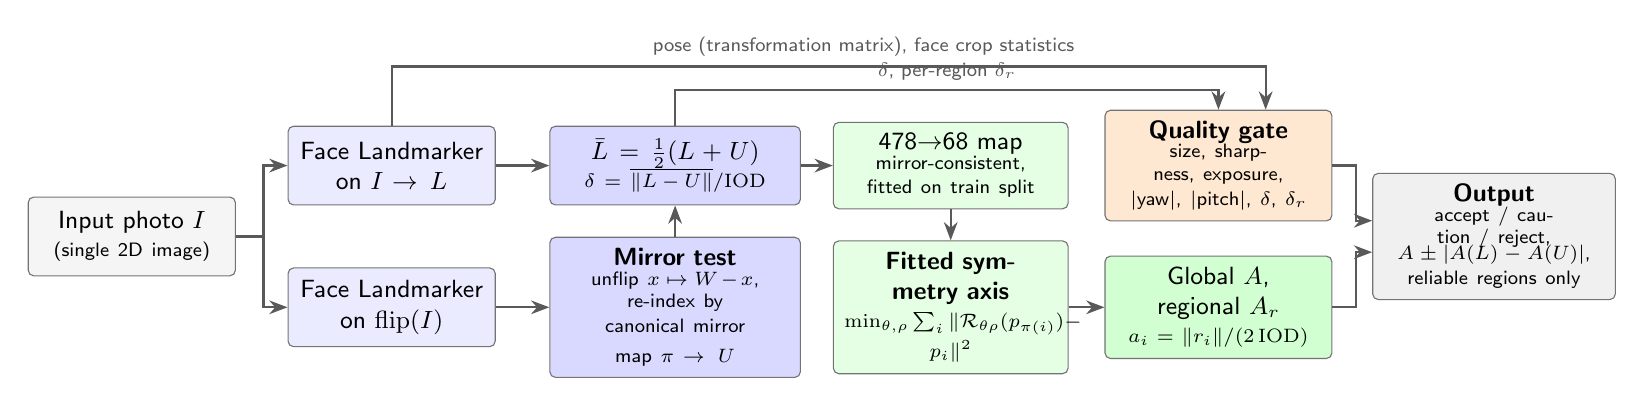
\begin{tikzpicture}[
  font=\sffamily\small, >=Stealth,
  box/.style={draw=black!55, rounded corners=2pt, fill=#1, align=center, inner sep=4pt,
              minimum height=1.0cm, text width=2.35cm},
  box/.default=white,
  arr/.style={->, thick, black!65},
  lab/.style={font=\sffamily\scriptsize, text=black!65, align=center}
]
% column 1: input
\node[box=black!4] (in) at (0,0) {Input photo $I$\\[-1pt]\scriptsize (single 2D image)};
% column 2: two detections
\node[box=blue!8]  (d1) at (3.3, 0.9) {Face Landmarker\\on $I$ $\rightarrow L$};
\node[box=blue!8]  (d2) at (3.3,-0.9) {Face Landmarker\\on $\mathrm{flip}(I)$};
% column 3: mirror test
\node[box=blue!15, text width=2.9cm] (mt) at (6.9,-0.9) {\textbf{Mirror test}\\[-1pt]\scriptsize unflip $x\!\mapsto\!W\!-\!x$, re-index by\\[-2pt]\scriptsize canonical mirror map $\pi$ $\rightarrow U$};
\node[box=blue!15, text width=2.9cm] (avg) at (6.9, 0.9) {$\bar L=\tfrac12(L+U)$\\[-1pt]\scriptsize $\delta=\overline{\|L-U\|}/\mathrm{IOD}$};
% column 4: 68 mapping + axis
\node[box=green!10, text width=2.7cm] (map) at (10.4, 0.9) {478$\rightarrow$68 map\\[-1pt]\scriptsize mirror-consistent,\\[-2pt]\scriptsize fitted on train split};
\node[box=green!10, text width=2.7cm] (ax) at (10.4,-0.9) {\textbf{Fitted symmetry axis}\\[-1pt]\scriptsize $\min_{\theta,\rho}\sum_i\|\mathcal R_{\theta\rho}(p_{\pi(i)})-p_i\|^2$};
% column 5: measures
\node[box=green!18, text width=2.6cm] (meas) at (13.8,-0.9) {Global $A$, regional $A_r$\\[-1pt]\scriptsize $a_i=\|r_i\|/(2\,\mathrm{IOD})$};
% gate
\node[box=orange!18, text width=2.6cm] (gate) at (13.8, 0.9) {\textbf{Quality gate}\\[-1pt]\scriptsize size, sharpness, exposure,\\[-2pt]\scriptsize $|$yaw$|$, $|$pitch$|$, $\delta$, $\delta_r$};
% output
\node[box=black!6, text width=2.8cm] (out) at (17.3,0) {\textbf{Output}\\[-1pt]\scriptsize accept / caution / reject,\\[-2pt]\scriptsize $A\pm|A(L)-A(U)|$,\\[-2pt]\scriptsize reliable regions only};

\draw[arr] (in.east) -- ++(0.35,0) |- (d1.west);
\draw[arr] (in.east) -- ++(0.35,0) |- (d2.west);
\draw[arr] (d2) -- (mt);
\draw[arr] (d1.east) -- (avg.west);
\draw[arr] (mt) -- (avg);
\draw[arr] (avg) -- (map);
\draw[arr] (map) -- (ax);
\draw[arr] (ax) -- (meas);
\draw[arr] (avg.north) -- ++(0,0.45) -| node[lab, pos=0.25, above]{$\delta$, per-region $\delta_r$} (gate.north);
\draw[arr] (d1.north) -- ++(0,0.75) -| node[lab, pos=0.27, above]{pose (transformation matrix), face crop statistics} ([xshift=6mm]gate.north);
\draw[arr] (gate.east) -- ++(0.3,0) |- ([yshift=2mm]out.west);
\draw[arr] (meas.east) -- ++(0.3,0) |- ([yshift=-2mm]out.west);
\end{tikzpicture}}
\caption{\textbf{Overview of the proposed quality-aware measurement (variant M3).}
The landmarker is run on the photo and on its mirror image. Because a horizontal flip only
swaps anatomical sides, an ideal detector returns the same geometry twice; the disagreement
$\delta$ is a ground-truth-free check of landmark reliability, and the average $\bar L$
cancels any left/right bias of the detector. Asymmetry is measured on the standard 68-point
layout with fixed anatomical pairs and a fitted (not assumed) symmetry axis, and a score is
only reported when the quality/pose gate does not reject the image.}
\label{fig:overview}
\end{figure*}


\Cref{fig:overview} shows the pipeline. Each step is described below, together with the
reason it is there.

\subsection{Landmarks and fixed bilateral correspondence}
\label{sec:corr}
\textbf{Detection.} We use the MediaPipe Face Landmarker (Tasks API, float16 model) in
image mode. It returns $L\in\mathbb{R}^{478\times2}$ in pixels and a $4{\times}4$
canonical-to-camera transformation matrix, from which we read yaw, pitch and roll (ZYX
Euler angles). \emph{Why:} it runs on CPU in real time, needs no training, and its mesh has
a \emph{fixed topology}, which makes anatomical correspondence possible.

\textbf{Mirror permutation $\pi$.} MediaPipe's canonical face model is exactly
left--right symmetric. Reflecting it ($x\!\mapsto\!-x$) and taking the nearest vertex
gives an involution $\pi$ on the 468 face vertices, with a maximum residual of $0$:
220 bilateral pairs and 28 midline vertices (iris points are paired explicitly). A
vertex is therefore always compared with its own anatomical twin.
\emph{Why not KD-tree matching:} prior tools~\cite{nashokan_facialasymmetry,
varghaei2025aesthetic} reflect each left-side vertex and take the \emph{nearest} right-side
vertex. In a dense mesh the nearest vertex is often a neighbour of the true twin, so the
matching absorbs part of the asymmetry it should measure. On LFPW, \kdWrong\% of KD-tree
matches are not the anatomical partner (\cref{fig:corr}).

\textbf{478$\to$68 mapping.} We report on the 300-W 68-point layout, whose bilateral pairs
are defined by the annotation protocol and for which expert annotations exist. For each
iBUG point $k$ and mesh vertex $v$ we compute $E_{kv}$, the median over the 810
\emph{training} images of $\|L_v-G_k\|/\mathrm{IOD}$, and choose, for each iBUG pair
$(a,b)$, the vertex $v^\star=\arg\min_v E_{av}+E_{b\pi(v)}$, setting $a\!\to\!v^\star$,
$b\!\to\!\pi(v^\star)$. Midline points are mapped to midline vertices. The resulting map
is \emph{mirror-consistent} by construction ($\pi\circ m = m\circ\pi_{68}$), so the
mapping itself cannot create asymmetry. On the test split it reduces the inner-51-point
NME from \nmeHandInner\% (a widely used hand-made map) to \nmeFitInner\% (median
\nmeFitInnerMed\%), and the jaw NME from \nmeHandJaw\% to \nmeFitJaw\%.

\subsection{Asymmetry with a fitted symmetry axis}
\label{sec:axis}
Let $p_i$ be the 68 points, $\pi$ their mirror permutation and
$\mathcal{R}_{\theta,\rho}(x)=x-2(n^\top x-\rho)\,n$ the reflection about the line
$n^\top x=\rho$, $n=(\cos\theta,\sin\theta)$. We fit the axis on the inner face
($\mathcal{I}$: brows, eyes, nose, mouth; 51 points):
\begin{equation}
(\theta^\star,\rho^\star)=\arg\min_{\theta,\rho}\sum_{i\in\mathcal{I}}
\bigl\|\mathcal{R}_{\theta,\rho}(p_{\pi(i)})-p_i\bigr\|^2,
\label{eq:axis}
\end{equation}
initialised in closed form from pair midpoints and pair directions, then refined with
Nelder--Mead. With residuals $r_i=\mathcal{R}_{\theta^\star\!,\rho^\star}(p_{\pi(i)})-p_i$,
\begin{equation}
a_i=\frac{\|r_i\|}{2\,\mathrm{IOD}},\qquad
A=\frac{1}{|\mathcal{I}|}\sum_{i\in\mathcal{I}}a_i,\qquad
A_r=\frac{1}{|r|}\sum_{i\in r}a_i ,
\label{eq:asym}
\end{equation}
where IOD is the outer-eye-corner distance (the 300-W normaliser). $a_i$ is the distance of
point $i$ from the nearest exactly mirror-symmetric shape, as a fraction of IOD, and we
report $100A$ (``\% IOD''). \emph{Why:} (i) the axis is estimated, not assumed. A vertical
line through two chosen landmarks makes any head roll, or any error in those two
landmarks, look like asymmetry. \Cref{eq:asym} is invariant to rotation, translation and
scale of the image (unit-tested). (ii) Unlike Procrustes superimposition, a pure
reflection cannot hide asymmetry in a glide component. (iii) The 17-point jaw contour is a
pose-dependent silhouette, so it is reported as a region but excluded from $A$.
For readability the app also shows $S=100/(1+\alpha A)$ with $\alpha$=\alphaIndex{}
(the training median, \trainMedian\% IOD, maps to 50). $S$ is only a monotone
re-expression of $A$, not a validated scale.

\begin{figure}[t]
\centering
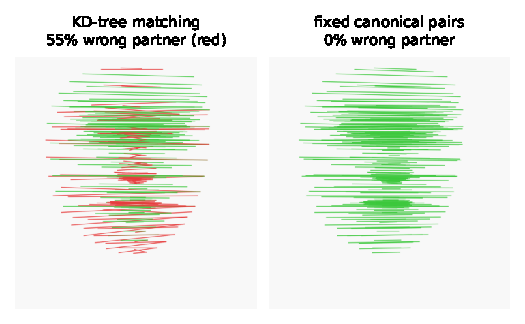
\includegraphics[width=\linewidth]{figures/correspondence.pdf}
\caption{\textbf{Correspondence matters.} Lines join each left-side vertex to its
partner for one test face (geometry only; see \cref{sec:ethics}). Left: baseline KD-tree
matching after reflection; red lines are matches that are not the anatomical twin.
Right: fixed pairs from the symmetric canonical model.}
\label{fig:corr}
\end{figure}

\subsection{The mirror test}
\label{sec:mirror}
We run the detector on $I$ and on its horizontal flip $I^{f}$. A point at $x'$ in $I^{f}$
lies at $W-x'$ in $I$ (MediaPipe uses continuous coordinates with pixel centres at
$i+\tfrac12$), and flipping swaps anatomical sides, so the vertex reported as $j$ in $I^{f}$
is vertex $\pi(j)$ of $I$:
\begin{equation}
U_{\pi(j)} = \bigl(W-L^{f}_{j,x},\;L^{f}_{j,y}\bigr).
\end{equation}
For an ideal detector $U\!=\!L$. We define the \emph{mirror inconsistency}
$\delta=\tfrac{1}{|\mathcal{I}|}\sum_{i\in\mathcal{I}}\|L_i-U_i\|/\mathrm{IOD}$ (and per region,
$\delta_r$), and measure asymmetry on the average $\bar L=\tfrac12(L+U)$.
\emph{Why:} the true asymmetry of a face does not change when the image is flipped, but
a detector's errors do not have to flip with it. The disagreement $\delta$ therefore
estimates landmark unreliability \emph{without ground truth}. MediaPipe exposes no
per-landmark confidence, so $\delta$ fills that gap. Averaging cancels any systematic
left/right bias of the detector, and $|A(L)-A(U)|$ is shown to the user as a stability
band. The cost is one extra detector pass (\runtime\,ms per image in total, including the
baseline's re-detection, on a 2-core 2.1\,GHz Xeon).

\subsection{Quality and pose gate}
\label{sec:gate}
The gate reads seven signals that the system can actually observe
(\cref{tab:thresholds}):
\textbf{face size} (IOD in pixels);
\textbf{sharpness}, $\log_{10}$ of the variance of the Laplacian~\cite{pertuz2013focus} on the face crop
resized to 256\,px width, so that it does not depend on face size;
\textbf{exposure}, the mean luma and the fraction of clipped pixels in the face crop;
\textbf{$|$yaw$|$, $|$pitch$|$} from the transformation matrix;
and the \textbf{mirror inconsistency} $\delta$.
In-plane roll is \emph{not} gated, because \cref{eq:axis} is invariant to it.
The worst signal decides accept / caution / reject, and every decision is shown with a
plain-language reason. A rejected image never shows a score unless the user explicitly
asks for it, and it is then labelled unreliable. In addition, a region whose
$\delta_r$ exceeds a training percentile is marked \emph{unreliable} and greyed out.

\textbf{Threshold policy} (fixed before looking at test results): pose and face-size limits
follow from the measurement's assumptions (yaw 10$^\circ$/20$^\circ$, pitch 15$^\circ$/25$^\circ$,
IOD 60/30\,px). Image-statistic limits are percentiles of the \emph{training} split: 2.5th
percentile of sharpness and of brightness for caution, and 90th/99th percentiles of
$\delta$. The test split is used only for evaluation.

\begin{table}[t]
\centering\footnotesize
\resizebox{\linewidth}{!}{\begin{tabular}{@{}llll@{}}
\toprule
Signal & caution & reject & source\\
\midrule
face size (IOD) & $<$ 60 px & $<$ 30 px & a priori\\
sharpness ($\log_{10}$ var. Lap.) & $<$ 1.4 & $<$ 0.756 & train pct.\\
mean luma (low) & $<$ 59.3 & $<$ 35 & train pct. / a priori\\
mean luma (high) & $>$ 164 & $>$ 225 & train pct. / a priori\\
clipped pixels & $>$ 0.364 & $>$ 0.6 & train pct. / a priori\\
$|$yaw$|$ & $>$ 10$^\circ$ & $>$ 20$^\circ$ & a priori\\
$|$pitch$|$ & $>$ 15$^\circ$ & $>$ 25$^\circ$ & a priori\\
mirror inconsistency $\delta$ & $>$ 0.0224 & $>$ 0.0489 & train pct.\\
per-region $\delta_r$ (validity) & \multicolumn{2}{l}{unreliable if $>$ 0.0444} & train pct.\\
\bottomrule
\end{tabular}
}
\caption{\textbf{Gate thresholds} (\texttt{configs/gate\_thresholds.json}).
``train pct.'': percentile of the \nTrainOk{} LFPW training faces.}
\label{tab:thresholds}
\end{table}

\subsection{Compared variants}
\label{sec:variants}
All variants use the \emph{same} detections of each image:
\textbf{M0} (baseline) is our re-implementation of~\cite{nashokan_facialasymmetry}: similarity
alignment of vertices 33/263 to fixed positions, re-detection, a vertical midline through
33/263, KD-tree reflected matching on all vertices, and the mean distance divided by face
width. That repository has no licence, so we re-implemented the method from its
description and code rather than copying it. Note that 33/263 are the \emph{outer} eye
corners, although the code comments call them inner corners.
\textbf{M1}: fixed 68-point pairs + fitted axis (\cref{sec:corr,sec:axis}).
\textbf{M2}: M1 + gate without $\delta$.
\textbf{M3} (full system): measurement on $\bar L$, gate with $\delta$, region validity.

\section{Experiments}
\label{sec:exp}

\subsection{Setup}
\textbf{Data.} We use LFPW~\cite{belhumeur2011lfpw} with the 300-W 68-point
re-annotation~\cite{sagonas2013_300w,sagonas2016_300w}, obtained from the Menpo
mirror~\cite{menpo_lfpw} (\cref{tab:data}). Following the 300-W protocol, which supplies a
face box, each image is cropped around the annotated face (landmark extent + 60\%);
many LFPW photos contain several people. The \textbf{train} split is used \emph{only} to
fit the 478$\to$68 map and to calibrate the gate. Every number below is computed on the
\textbf{test} split. WFLW~\cite{wu2018lab} was our first choice for its attribute subsets,
but its Google-Drive-hosted images were unreachable from our compute environment. The code
reads any 68-point \texttt{.pts} dataset.

\begin{table}[t]
\centering\footnotesize
\begin{tabular}{@{}lccl@{}}
\toprule
Split & Images & Faces detected & Used for\\
\midrule
LFPW train & 811 & 810 & 478$\to$68 map, gate calibration\\
LFPW test & 224 & 224 & all evaluation (clean)\\
Perturbed test & 5{,}824 & 5{,}730 & robustness (26 settings $\times$ 224)\\
\bottomrule
\end{tabular}
\caption{\textbf{Data.} 68 manual landmarks per face; research-use licence (300-W).}
\label{tab:data}
\end{table}

\textbf{Reference without symmetry labels.} No public dataset has ground-truth symmetry
ratings. We therefore compute the \emph{same} measure (\cref{eq:asym}) from the expert
68-point annotations, $A_{ref}$, and evaluate how well each detector-based measure agrees
with it (Spearman $\rho$, Pearson $r$, MAE). $A_{ref}$ is not ``true'' asymmetry: it
contains annotator noise and the same 2D/pose limitations (\cref{sec:discussion}). It is
the best available reference for \emph{the measurement} we want to automate.

\textbf{Perturbations} (deterministic, applied to all 224 test faces): brightness
$\times\{0.25,0.4,0.6,1.5,2,2.5\}$; Gaussian blur $\sigma\!=\!s\cdot\mathrm{IOD}/100$,
$s\!\in\!\{1,2,4,6,8\}$; a grey box over one eye, the nose or the mouth (annotation box
+35\%); in-plane rotation $\pm\{5,10,20,30\}^\circ$ on an enlarged canvas; and downscaling
$\times\{0.5,0.3,0.2,0.12\}$. The face is unchanged, so $A_{ref}$ is unchanged too.

\textbf{Metrics.} \emph{Drift}: median $|$score(perturbed)$-$score(clean)$|$ divided by the
clean between-subject SD of that variant. This is scale-free, so M0 (face-width units) and
M1/M3 (IOD units) can be compared. \emph{Reported}: fraction of images not rejected.
\emph{Silent failure}: fraction of images whose score is \emph{reported} but has
$|A-A_{ref}|>1\%$ IOD (about twice the clean MAE, fixed a priori). This is the failure a
gate must prevent. For M0, MAE and silent failure are undefined because its units differ
from those of $A_{ref}$.
\textbf{Implementation:} Python 3.13, MediaPipe 0.10.32, OpenCV 5.0, NumPy/SciPy, Streamlit
1.66; CPU only. All tables and figures are generated by scripts from the saved CSVs.

\begin{figure*}[t]
\centering
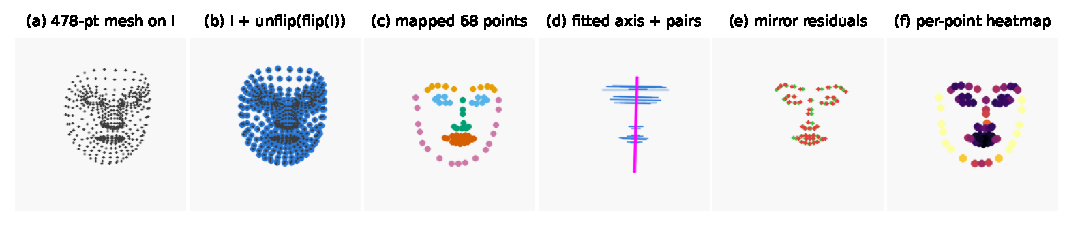
\includegraphics[width=\textwidth]{figures/pipeline_examples.pdf}
\caption{\textbf{Intermediate outputs for one test face}, drawn as geometry only.
(a) mesh on $I$; (b) mesh on $I$ (black) and unflipped mesh from $\mathrm{flip}(I)$ (blue),
almost coincident here ($\delta$ small); (c) mapped 68 points coloured by region;
(d) bilateral pairs and the fitted axis (magenta); (e) each point (green) and the
reflection of its partner (red); (f) per-point $a_i$ (bright = larger).}
\label{fig:pipeline}
\end{figure*}

\subsection{E1--E3: agreement with the annotation-based reference}
\Cref{tab:agree} and \cref{fig:agree} answer the first question: does the system measure
what we intend? The re-implemented baseline reaches $\rho$=\rhoMzero{}, or \rhoMzeroNoAlign{}
without its alignment step. Replacing only its KD-tree matching with the fixed canonical
pairs, keeping the same detections, mesh and midline, raises $\rho$ to \rhoMzeroFixed{}.
\emph{Correspondence is the dominant error source in the baseline.} The 68-point measure
with the fitted axis reaches \rhoMone{} (MAE \maeMone\% IOD), and mirror averaging reaches
\rhoMthree{}.

\begin{table}[t]
\centering\footnotesize
\setlength{\tabcolsep}{3pt}
\resizebox{\linewidth}{!}{\begin{tabular}{@{}lccc@{}}
\toprule
Measure ($n$=224) & $\rho$ & $r$ & MAE\\
\midrule
M0 baseline~\cite{nashokan_facialasymmetry} (KD-tree, vert.\ midline) & 0.823 & 0.762 & --\\
\quad M0 w/o alignment & 0.614 & 0.630 & --\\
\quad M0 + fixed pairs (no KD-tree) & 0.931 & 0.903 & --\\
M1: 68-pt pairs + fitted axis & 0.938 & 0.951 & 0.45\\
M3: M1 + mirror averaging & 0.947 & 0.957 & 0.45\\
\bottomrule
\end{tabular}
}
\caption{\textbf{Agreement with $A_{ref}$} on the clean LFPW test set (E1/E2): Spearman $\rho$, Pearson $r$, MAE in \% IOD. All rows
use identical detections.}
\label{tab:agree}
\end{table}

\begin{figure}[t]
\centering
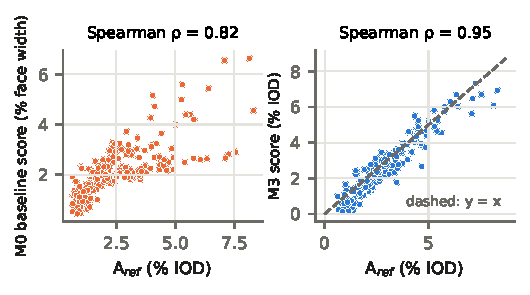
\includegraphics[width=\linewidth]{figures/agreement.pdf}
\caption{\textbf{Detector-based score vs.\ annotation-based reference} (224 test faces).
Left: baseline M0. Right: proposed M3. Points below $y\!=\!x$ show that the detector
under-estimates asymmetry.}
\label{fig:agree}
\end{figure}

\textbf{Regional analysis (E3, \cref{tab:regions}).} Regional agreement is lower than
global agreement ($\rho$ 0.84--0.98) because each region has fewer points. A systematic effect
appears: detector-based asymmetry is \emph{smaller} than annotation-based asymmetry, by
\shrinkGlobal\% globally and \shrinkMouth\% at the mouth (Wilcoxon $p<$0.01 except for the
brows, $p$=\pBrows{}). MediaPipe regresses a mesh with a strong shape prior, and this
pulls atypical (asymmetric) shapes towards the symmetric template. Part of the gap may also
be annotator noise, which inflates $A_{ref}$. Users should read detector-based regional
values as conservative.

\begin{table}[t]
\centering\footnotesize
\setlength{\tabcolsep}{3pt}
\resizebox{\linewidth}{!}{\begin{tabular}{@{}lcccccc@{}}
\toprule
 & \multicolumn{2}{c}{Spearman $\rho$} & \multicolumn{2}{c}{MAE (\% IOD)} & \multicolumn{2}{c}{mean A (\% IOD)}\\
\cmidrule(lr){2-3}\cmidrule(lr){4-5}\cmidrule(lr){6-7}
Region & M1 & M3 & M1 & M3 & ref & M3\\
\midrule
Brows & 0.840 & 0.848 & 0.76 & 0.76 & 2.85 & 2.80$^{\dagger}$\\
Eyes & 0.882 & 0.895 & 0.59 & 0.56 & 2.25 & 2.08\\
Nose & 0.912 & 0.914 & 0.87 & 0.86 & 3.90 & 3.53\\
Mouth & 0.876 & 0.889 & 0.54 & 0.56 & 1.86 & 1.36\\
Jaw & 0.974 & 0.977 & 1.61 & 1.60 & 11.73 & 10.44\\
\midrule
Global (inner 51) & -- & -- & -- & -- & 2.51 & 2.19\\
\bottomrule
\end{tabular}
}
\caption{\textbf{Regional agreement and shrinkage} (E3). Right block: mean asymmetry from
annotations vs.\ M3. $^{\dagger}$difference not significant (Wilcoxon $p\geq$0.01).}
\label{tab:regions}
\end{table}

\subsection{E8: head pose confounds 2D asymmetry}
\Cref{fig:pose} and \cref{tab:pose} show the strongest effect we observed. Even computed from
\emph{expert annotations}, 2D asymmetry follows $|$yaw$|$ almost monotonically
($\rho$=\rhoYawRef{}), from \yawLow\% IOD below 5$^\circ$ to \yawHigh\% above 20$^\circ$.
A turned head foreshortens one half of the face, and no 2D reflection can undo that. This
is a property of the \emph{quantity}, not of the detector. The detector's error relative to
$A_{ref}$ barely changes with yaw (\cref{tab:pose}), which is why a gate trained to predict
detector error would miss it. Restricting to gate-accepted images lowers the correlation to
$\rho$=\rhoYawRefAcc{}, but it does not remove it. LFPW is an in-the-wild set whose test
faces mostly have $|$yaw$|>$5$^\circ$. For a frontal capture the remaining pose effect is small,
but a ``symmetry score'' computed from an arbitrary selfie mostly measures head pose.

\begin{figure}[t]
\centering
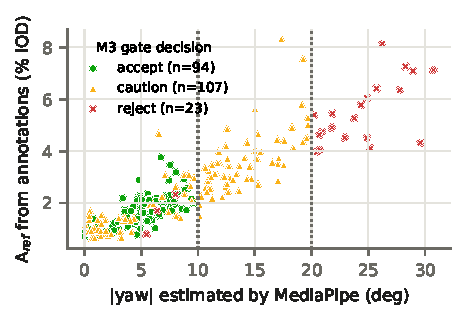
\includegraphics[width=0.95\linewidth]{figures/pose_confound.pdf}
\caption{\textbf{Asymmetry from expert annotations vs.\ estimated $|$yaw$|$} (E8), coloured
by the M3 gate decision. Dotted lines: caution (10$^\circ$) and reject (20$^\circ$) limits.}
\label{fig:pose}
\end{figure}

\begin{table}[t]
\centering\footnotesize
\resizebox{\linewidth}{!}{\begin{tabular}{@{}lccccc@{}}
\toprule
$|$yaw$|$ (deg) & n & A$_{ref}$ & M1 & $|$err$|$ M3 & NME\\
\midrule
0-5 & 77 & 1.20 & 0.80 & 0.47 & 3.03\\
5-10 & 67 & 2.14 & 1.86 & 0.40 & 5.51\\
10-20 & 60 & 3.60 & 3.41 & 0.42 & 3.32\\
$\geq$20 & 20 & 5.50 & 5.42 & 0.57 & 4.13\\
\bottomrule
\end{tabular}
}
\caption{\textbf{Pose strata} (E8, test set; values in \% IOD). Each image is
observed once, so the strata contain \emph{different} people, not the same face at several poses.}
\label{tab:pose}
\end{table}

\subsection{The mirror test detects bad landmarks without labels}
Across test images, $\delta$ correlates with the true landmark error (inner-51 NME,
$\rho$=\rhoMirrorNme{}). As a ranking signal for discarding images (\cref{fig:rc}, left),
it lowers the area under the NME risk--coverage curve from \aurcRandom{} (random) to
\aurcMirror{} (oracle: \aurcOracle{}), closing \gapClosed\% of the gap to the oracle. The
image-quality gate risk alone reaches \aurcGateTwo{}. $\delta$ predicts the
\emph{asymmetry} error much less well ($\rho$=\rhoMirrorErr{}; AURC \aurcAsymMirror{}
vs.\ \aurcAsymRandom{} random; \cref{fig:rc}, right). On clean photos, most landmark
errors are shared by the two sides of the face and cancel in $A$. The gate's value for
asymmetry shows up under degradation (\cref{sec:robust}).

\begin{figure}[t]
\centering
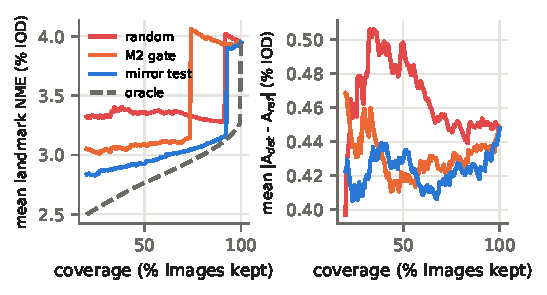
\includegraphics[width=\linewidth]{figures/risk_coverage.pdf}
\caption{\textbf{Risk--coverage on the clean test set.} Images are kept in order of
increasing risk; the y-axis is the mean error of the kept set (lower is better).
Left: landmark NME. Right: asymmetry error $|A_{det}-A_{ref}|$.}
\label{fig:rc}
\end{figure}

\subsection{E4--E7, E9: robustness and ablation}
\label{sec:robust}
\Cref{fig:robust} and \cref{tab:ablation} summarise 5{,}824 perturbed measurements.
MediaPipe is remarkably robust: it still finds a face in $\geq$\detMin\% of the images in
every setting (lowest: blur $s$=8). The danger is therefore not a missing result but a
\emph{plausible-looking wrong} one. Without a gate (M1), \silentPoolOne\% of all perturbed
measurements are silent failures, rising to \silentBlurOne\% under blur. The gate (M2/M3)
lowers this to \silentPoolTwo\%/\silentPoolThree\% (blur: \silentBlurThree\%; downscaling:
\silentDownOne\%$\to$\silentDownThree\%). The cost is coverage: \covPoolThree\% of perturbed
and \covCleanThree\% of clean images still receive a score. On clean images silent
failures fall from \silentCleanOne\% to \silentCleanThree\%.
\textbf{Mirror averaging} lowers the median drift from \driftPoolOne{} to \driftPoolThree{}
SD (\driftReduction\% less, pooled) and helps under \emph{every} perturbation type.
\textbf{In-plane rotation} (E7): a vertical-midline measure without alignment drifts by up
to \rotNoAlignMax{} SD at 30$^\circ$. The baseline's align-and-re-detect step fixes this, at
the cost of a second detection. The fitted axis achieves the same stability (M3 $\leq$
\rotMthreeMax{} SD) with no re-detection.

\begin{figure*}[t]
\centering
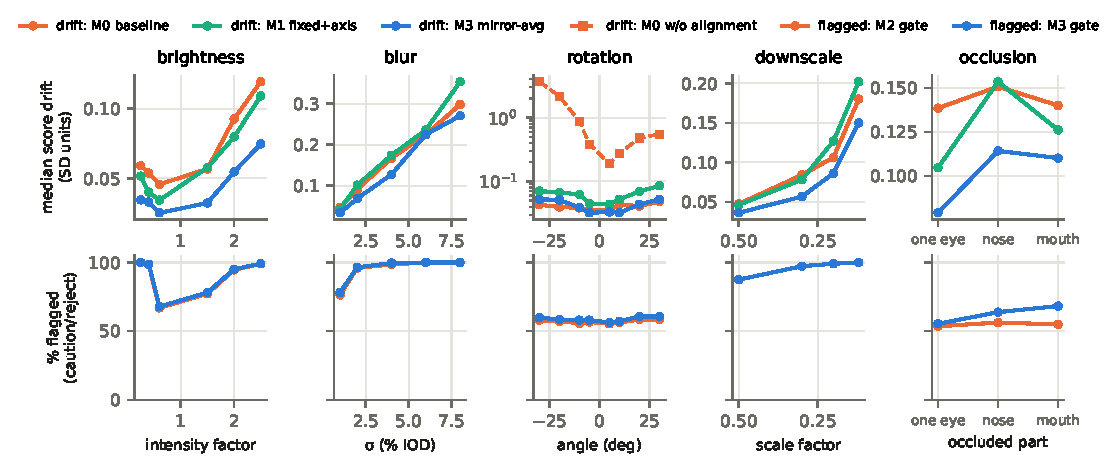
\includegraphics[width=0.92\textwidth]{figures/robustness.pdf}
\caption{\textbf{Controlled perturbations} (E4--E7; 224 test faces per point). Top:
median score drift in units of the clean between-subject SD (rotation panel in log scale;
dashed: vertical-midline baseline without alignment). Bottom: share of images the gate
flags as caution or reject.}
\label{fig:robust}
\end{figure*}

\begin{table}[t]
\centering\scriptsize
\setlength{\tabcolsep}{2.2pt}
\resizebox{\linewidth}{!}{\begin{tabular}{@{}llcccccc@{}}
\toprule
Setting & Var. & n & Reported & Accepted & $\rho$ & Silent fail. & Drift\\
 & & & (\%) & (\%) & vs ref & (\%) $\downarrow$ & (SD) $\downarrow$\\
\midrule
Clean test & M0 & 224 & 100.0 & 100.0 & 0.823 & -- & --\\
 & M1 &  & 100.0 & 100.0 & 0.938 & 5.8 & --\\
 & M2 &  & 90.2 & 43.3 & 0.921 & 4.9 & --\\
 & M3 &  & 89.7 & 42.0 & 0.932 & 4.0 & --\\
\midrule
Perturbed, pooled & M0 & 5824 & 98.4 & 98.4 & 0.814 & -- & 0.070\\
 & M1 &  & 98.4 & 98.4 & 0.921 & 8.1 & 0.076\\
 & M2 &  & 64.0 & 22.6 & 0.918 & 3.4 & =\\
 & M3 &  & 63.2 & 21.0 & 0.927 & 3.6 & 0.054\\
\midrule
\quad blur & M0 & 1120 & 94.0 & 94.0 & 0.787 & -- & 0.131\\
 & M1 &  & 94.0 & 94.0 & 0.870 & 14.4 & 0.130\\
 & M2 &  & 37.0 & 5.8 & 0.903 & 2.7 & =\\
 & M3 &  & 35.6 & 5.2 & 0.919 & 2.3 & 0.099\\
\midrule
\quad downscale & M0 & 896 & 98.7 & 98.7 & 0.821 & -- & 0.087\\
 & M1 &  & 98.7 & 98.7 & 0.909 & 9.2 & 0.097\\
 & M2 &  & 33.5 & 4.0 & 0.919 & 1.8 & =\\
 & M3 &  & 33.4 & 4.0 & 0.927 & 1.9 & 0.066\\
\midrule
\quad brightness & M0 & 1344 & 99.5 & 99.5 & 0.818 & -- & 0.065\\
 & M1 &  & 99.5 & 99.5 & 0.936 & 5.8 & 0.056\\
 & M2 &  & 62.8 & 10.6 & 0.927 & 2.8 & =\\
 & M3 &  & 62.4 & 10.2 & 0.940 & 2.7 & 0.037\\
\midrule
\quad occlusion & M0 & 672 & 98.8 & 98.8 & 0.804 & -- & 0.142\\
 & M1 &  & 98.8 & 98.8 & 0.919 & 8.8 & 0.124\\
 & M2 &  & 87.9 & 45.1 & 0.900 & 6.2 & =\\
 & M3 &  & 85.1 & 37.5 & 0.911 & 6.0 & 0.098\\
\midrule
\quad rotation & M0 & 1792 & 100.0 & 100.0 & 0.825 & -- & 0.039\\
 & M1 &  & 100.0 & 100.0 & 0.944 & 5.2 & 0.059\\
 & M2 &  & 88.1 & 43.0 & 0.924 & 4.0 & =\\
 & M3 &  & 87.7 & 41.4 & 0.928 & 4.9 & 0.040\\
\bottomrule
\end{tabular}
}
\caption{\textbf{Ablation} (E9). Reported = not rejected; Accepted = no caution.
Silent fail.: reported \emph{and} $|A-A_{ref}|>$1\% IOD. Drift: median, in clean-SD units
(``='': same score as M1).}
\label{tab:ablation}
\end{table}

\textbf{Gate behaviour on clean photos.} On the clean test set M3 accepts \pAccept\%,
cautions \pCaution\% and rejects \pReject\% of the faces. The mean NME of accepted faces
is \nmeAccept\% vs.\ \nmeCaution\% for caution. \Cref{tab:reasons} lists the triggers;
pose dominates, consistent with E8. \Cref{fig:gate} shows one face per decision.

\begin{table}[t]
\centering\footnotesize
\begin{minipage}{0.45\linewidth}\centering
\resizebox{\linewidth}{!}{\begin{tabular}{@{}lcc@{}}
\toprule
Signal & caution & reject\\
\midrule
$|$yaw$|$ & 60 & 20\\
$|$pitch$|$ & 41 & 2\\
mirror inconsistency $\delta$ & 12 & 1\\
face size (IOD) & 16 & 0\\
over-exposure & 10 & 0\\
sharpness & 7 & 0\\
several faces & 6 & 0\\
clipped pixels & 4 & 0\\
under-exposure & 3 & 0\\
\bottomrule
\end{tabular}
}
\end{minipage}\hfill
\begin{minipage}{0.53\linewidth}
\caption{\textbf{Which signal triggered the gate} on the 224 clean test faces (one image can
trigger several).}
\label{tab:reasons}
\end{minipage}
\end{table}

\begin{figure}[t]
\centering
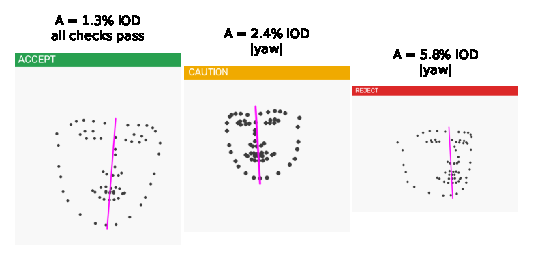
\includegraphics[width=\linewidth]{figures/gate_examples.pdf}
\caption{\textbf{Gate decisions} for three test faces (the median-$|$yaw$|$ face of each
class), drawn as landmarks + fitted axis.}
\label{fig:gate}
\end{figure}

\textbf{Region validity under occlusion: a negative result.} When the nose or the mouth
is occluded, $\delta_r$ marks that region unreliable in \occNose\% and \occMouth\% of the
faces, against \occNoseOther\% and \occMouthOther\% for the other regions. When an
\emph{eye} is occluded it does so in only \occEye\% of faces. MediaPipe fills in the
hidden eye from its shape prior, and does so consistently in both the original and the
mirror image. The mirror test detects \emph{inconsistent} landmarks, not
\emph{confidently invented} ones. Occlusion needs an appearance-based check (future work).

\section{Discussion and Limitations}
\label{sec:discussion}

\paragraph{What worked.} Two changes give most of the gain over the public baseline: using
the anatomical correspondence that the mesh already provides, and estimating the symmetry
axis instead of assuming it. The mirror test is cheap, needs no labels, and gives the
system a landmark-reliability signal that MediaPipe does not expose. The gate turns many
silent failures into explicit refusals.

\paragraph{What did not.} The mirror test cannot detect an occluded eye that the detector
fills in consistently. On clean photos the gate does not predict small asymmetry errors
better than chance, because those errors are dominated by symmetric landmark noise and
by the detector's shrinkage towards symmetry.

\paragraph{Limitations.}
\begin{itemize}[leftmargin=*,itemsep=1pt,topsep=2pt]
\item \textbf{2D only.} A photo is a projection. Yaw and pitch change the measured value
(E8), and the gate can only limit, not remove, that effect. Camera perspective at selfie
distance is not modelled.
\item \textbf{Reference, not ground truth.} $A_{ref}$ uses expert landmarks, which contain
annotator noise, and is subject to the same projection effects. We have no human
symmetry ratings, and a validated perceptual or clinical scale was out of scope.
\item \textbf{Dataset.} LFPW is small (224 test faces), in the wild and mostly non-frontal,
and each identity appears once, so the pose strata are not paired. MediaPipe's training
data is not public and could overlap with LFPW, so its NME here is not an independent
benchmark claim. We use it only to compare mappings and gate signals.
\item \textbf{Thresholds} are percentiles of one training distribution. A different camera
or population would need re-calibration (\texttt{calibrate\_gate.py}).
\item \textbf{Expression} is not controlled. A smile is asymmetric by nature, so the app
asks for a neutral expression.
\end{itemize}

\paragraph{Ethics and privacy.}
\label{sec:ethics}
The output is a geometric indicator. It says nothing about health, identity or
attractiveness, and the app states this. Dataset images are used under their research
licence and are neither redistributed in the repository nor reproduced in this report.
Figures draw landmark geometry on a blank canvas. The app processes uploads in memory and
stores nothing.

\section{Conclusion and Future Work}
We built and evaluated a quality-aware facial asymmetry system that reports a measurement
only when the image supports it. On LFPW it tracks an annotation-based reference much more
closely than a re-implemented public baseline ($\rho$ \rhoMthree{} vs.\ \rhoMzero{}). Its
mirror test flags unreliable landmarks without labels, and its gate cuts silent failures
under degradation from \silentPoolOne\% to \silentPoolThree\%. The study also gives a
practical warning: in uncontrolled photos, head yaw explains most of the measured 2D
asymmetry. Future work: frontalisation with the detector's 3D landmarks, evaluated on a
dataset with ground-truth pose (\eg AFLW2000-3D~\cite{zhu2016aflw2000}); appearance-based
occlusion detection; WFLW's attribute subsets; and a small consented, multi-pose capture of
the same people with human symmetry ratings.


{\small
\bibliographystyle{ieee_fullname}
\bibliography{main}
}

\clearpage
\appendix
\section{Team Contributions}
\label{sec:contrib}
\begin{itemize}[leftmargin=*,itemsep=2pt,topsep=2pt]
\item \textbf{Prutha Vinay (230807)}: project coordination; symmetry geometry engine
(fitted axis, mirror test, \texttt{geometry.py}, \texttt{pipeline.py}); integration and
repository maintenance.
\item \textbf{Ankit Yadav (230150)}: dataset pipeline (LFPW/300-W loading, face crops), the
mirror-consistent 478$\to$68 mapping fit and the landmark (NME) evaluation.
\item \textbf{Ashish Porwal (230229)}: quality/pose gate design and calibration
(\texttt{quality.py}, \texttt{calibrate\_gate.py}); perturbation experiments E4--E7.
\item \textbf{Mahi Mittal (230617)}: Streamlit application and user interface,
visualisation module and paper figures.
\item \textbf{Pankaj Kumar (230733)}: literature and repository audit, re-implementation
of the baseline (M0), ablation analysis and report/presentation writing.
\end{itemize}
All members reviewed the results and the report.

\section{Code, Data and Resource Links}
\textbf{Project repository:} \repo\\
Run: \texttt{pip install -r requirements.txt}; \texttt{streamlit run app.py}.
Reproduce all results: see \texttt{README.md} (\texttt{experiments/} scripts in order).

\noindent\textbf{Datasets.}
LFPW/300-W: \url{https://ibug.doc.ic.ac.uk/resources/300-W/};
annotation scheme: \url{https://ibug.doc.ic.ac.uk/resources/facial-point-annotations/};
mirror used: \url{https://github.com/menpo/lfpw-train}, \url{https://github.com/menpo/lfpw-test};
WFLW (considered): \url{https://github.com/wywu/LAB};
CelebA (considered): \url{https://mmlab.ie.cuhk.edu.hk/projects/CelebA.html}.

\noindent\textbf{Repositories and tools.}
MediaPipe Face Landmarker: \url{https://developers.google.com/edge/mediapipe/solutions/vision/face_landmarker/python};
canonical face model: \url{https://github.com/google-ai-edge/mediapipe/tree/master/mediapipe/modules/face_geometry/data};
baseline method: \url{https://github.com/nashokan/FacialAsymmetry};
\url{https://github.com/varghaei/face-aesthetics-analysis};
\url{https://github.com/yousrajnahi/Facial-symmetry-estimation};
\url{https://github.com/irimidlab/irimid};
CVPR author kit: \url{https://github.com/cvpr-org/author-kit}.
No code was copied from the audited repositories (none has a licence file); the baseline
was re-implemented from its documented method.

\section{Complete Source Code}
\label{sec:code}
The complete source code is listed below and is also available in the repository. Unit
tests: \texttt{tests/test\_geometry.py} (15 tests, all passing).

\onecolumn
\subsection*{src/fsm/mesh.py}\lstinputlisting{code/src/fsm/mesh.py}
\subsection*{src/fsm/geometry.py}\lstinputlisting{code/src/fsm/geometry.py}
\subsection*{src/fsm/detector.py}\lstinputlisting{code/src/fsm/detector.py}
\subsection*{src/fsm/quality.py}\lstinputlisting{code/src/fsm/quality.py}
\subsection*{src/fsm/pipeline.py}\lstinputlisting{code/src/fsm/pipeline.py}
\subsection*{src/fsm/data.py}\lstinputlisting{code/src/fsm/data.py}
\subsection*{src/fsm/viz.py}\lstinputlisting{code/src/fsm/viz.py}
\subsection*{app.py}\lstinputlisting{code/app.py}
\subsection*{experiments/common.py}\lstinputlisting{code/experiments/common.py}
\subsection*{experiments/cache\_detections.py}\lstinputlisting{code/experiments/cache_detections.py}
\subsection*{experiments/fit\_mp68\_mapping.py}\lstinputlisting{code/experiments/fit_mp68_mapping.py}
\subsection*{experiments/calibrate\_gate.py}\lstinputlisting{code/experiments/calibrate_gate.py}
\subsection*{experiments/run\_clean\_eval.py}\lstinputlisting{code/experiments/run_clean_eval.py}
\subsection*{experiments/run\_perturbations.py}\lstinputlisting{code/experiments/run_perturbations.py}
\subsection*{experiments/summarize\_perturbations.py}\lstinputlisting{code/experiments/summarize_perturbations.py}
\subsection*{experiments/make\_figures.py}\lstinputlisting{code/experiments/make_figures.py}
\subsection*{experiments/make\_tables.py}\lstinputlisting{code/experiments/make_tables.py}
\subsection*{tests/test\_geometry.py}\lstinputlisting{code/tests/test_geometry.py}


\end{document}
